\chapter{Simulation Workflow}
\label{chap:workflow}

%%%%%%%%%%%%%%%%%%%%%%%%%%%%%%%%%%%%%%%%%%%%%%%%%%%%%%%%%%%%%%%%%%%%%%%%%%%%%%%%
\section{A Simulation Triad}
\label{chap3:triad}

This thesis investigates Monte Carlo as a means to generate multi-group cross sections for fine mesh transport codes. This work required the development of a ``simulation triad'' encompassing three primary codes. First, the OpenMC Monte Carlo code~\cite{romano2013openmc} was utilized to generate \ac{MGXS} as described in Sec.~\ref{sec:chap3-mgxs-gen}. Second, the \ac{MGXS} were used by the OpenMOC \ac{MOC} code~\cite{boyd2014openmoc} for deterministic multi-group transport calculations. Finally, the OpenCG library~\cite{boyd2015opencg} enabled the processing and transfer of tally data on combinatorial geometry (CG) meshes between OpenMC and OpenMOC. In addition, a significant amount of infrastructural code was developed to process the results produced by OpenMC and OpenMOC. This chapter describes the author's contributions to each component code in the simulation triad to support the objectives of this thesis -- namely, the evaluation of intrinsic bias in \ac{MGXS} for fine mesh transport, and the development of a novel metholodogy for spatial homgenization based on unsupervised clustering. An overview of the OpenMC, OpenMOC, and OpenCG codes, along with the features added to each code for this thesis, are presented in Secs.~\ref{sec:chap3-openmc},~\ref{sec:chap3-openmoc}, and~\ref{sec:chap3-opencg}, respectively.

%The infrastructural code framework was developed using the Python programming language due to its flexibility and ease of use, as well as its extensive ecosystem of open source packages for high-performance data analysis.

% including a Monte Carlo code, deterministic multi-group transport code, and the infrastructural code to tie the pieces together. 

%first paragraph: overview of codes
%-openmc as the monte carlo code
%-openmoc as deterministic multi-group code
%-opencg as the driver for CSG processing
%-python to tie it all together into a single framework

%Much of the code development for this thesis was motivated by the need to perform analysis of large tally datasets produced by OpenMC for \ac{MGXS} generation. The approach to spatial homogenization with unsupervised clustering requires the calculation of microscopic \ac{MGXS} for each nuclide in each spatial region (\textit{e.g.}, fuel pin) across an entire reactor core. For a \ac{PWR} consisting of $\sim$50,000 fuel pins of depleted fuel with $\sim$300 nuclides, subdivided into 100 

%second paragraph: big data -> perhaps this should be in the motivation above?
%-explain/assume the need to tally across each spatial mesh zone
%-need to process large amounts of tally data
%-BEAVRS core figures for motivation
%-bulletize requirements?
%  -\# nuclides, \# tally regions, \# groups => data size
  
%third paragraph: requirements for software
%-processing/transferring lots of data
%  -requires a robust and scalable framework to ``glue'' triad together
%-requires extensions to each code

%third paragraph: outline following sections
%-openmc
%-openmoc
%-opencg


%%%%%%%%%%%%%%%%%%%%%%%%%%%%%%%%%%%%%%%%%%%%%%%%%%%%%%%%%%%%%%%%%%%%%%%%%%%%%%%%
\section{OpenMC}
\label{sec:chap3-openmc}

The OpenMC code is a continuous energy Monte Carlo neutron transport code~\cite{romano2013openmc} with support for general constructive solid geometry models. OpenMC was initially created by Romano for his PhD thesis~\cite{romano2013parallel} to explore novel parallel algorithms for high-performance computing architectures. The code was released with the MIT open source license, and has attracted growing interest as platform for development of new physics methods and computational algorithms. Although this thesis could have plausibly used any continuous energy \ac{MC} neutron transport code, this author chose OpenMC for its general and extensible implementation, excellent parallel scalability, and open source license agreement which permits the modification of its codebase. The general physics and computational methods used in OpenMC will not be detailed here since they are well documented in the literature. The interested reader is referred to the online code manual~\cite{openmc2016manual} for further information.

%first paragraph: introduce OpenMC
%-history
%-high-level overview: CE, parallel perf., open source
%-not repeating MC theory, point to manual

second paragraph: motivation for big data MC
-condense paragraphs from PHYSOR paper intro
-parallelism is not enough (cite nick's papers)
-flat ASCII files suck
-generalized data model needed

third paragraph: pillars for approach
-re-use three pillars from OpenMC big data paper
  -expressive input
  -managed execution
  -seamless processing

fourth paragraph: outline
-python api
  -tally arithmetic, pandas
-distributed cell tallies
-openmc.mgxs module

%%%%%%%%%%%%%%%%%%%%%%%
\subsection{Python API}
\label{sec:chap3-py-api}

Big data OpenMC~\cite{boyd2016bigdata}

first paragraph: motivation (first paragraph in BD paper)
-facilitate input generation and downstream tally data processing
-tightly couple these processes
-important to have flexible handle on the geometry for high-fidelity spatial tallies
-expose OpenMC to extensive ecosystem of Python packages

second paragraph: input generation (second paragraph in BD paper)
-XML is human and machine readable
-relate back to MGXS generation
-cumbersome

third paragraph: data processing, OO (third paragraph in BD paper)
-OO with extensible class definitions
-flexible objects for data processing
-reconstruct geometry/materials objects from HDF5 statepoints
-allows for very flexible data processing
  -don't spend 95+\% of time coming up with ways to parse ASCII text output files


%%%%%%%%%%%%%%%%%%%%%%%%%%%%%%%%
\subsubsection{Tally Arithmetic}
\label{sec:chap3-tally-arithmetic}

-take from Big Data paper!!!
-look at jupyter notebooks
-need to describe statepiont/summary file structure?

first paragraph: motivate with MGXS
-need to combine tallies for MGXS
-want to propagate uncertainties
-want fast, efficient scheme to do this
  -i.e., vectorize across groups, nuclides, and esp. spatial tally zones

second paragraph: tally arithmetic as an OO solution
-take paragraph from BD paper
-operator overloading
-derived tallies
-chain operations together
-recall assumption of independent random variables
-need to go into detail about crossfilters, etc.?
-tally summation/averaging across bins

third paragraph: aggregation (slicing/merging)
-tally slicing and merging
-mention overhead associated with lots of tallies
-but nice for user to 1) create and 2) process lots of distinct tally objects
  -create lots of distinct tallies in Python input
  -automatically merge them for OpenMC XML input and runtime efficiency
  -construct tally objects from HDF5 statepoints
  -slice tallies apart again for processing
-operations use NumPy to efficiently create derived sliced/merged tallies

third paragraph: tie back to MGXS
-use tally arithmetic to compute MGXS from basic tallies (sliced/merged
-encapsulate MGXS in derived tally containers
-slicing/merging can be used to slice tallies apart by nuclide, group, domain, etc.
  -necessary for machine learning by nuclide, group, domain, etc.
  -use tally summation/averaging with ML output
  -use tally merging to re-assembly MGXS from outputs of ML algorithms

%%%%%%%%%%%%%%%%%%%%%%%%%%%%%%%%%
\subsubsection{Pandas DataFrames}
\label{sec:chap3-pandas-df}

Pandas~\cite{mckinney2010pandas}
-take from Big Data paper!!!
-look at jupyter notebooks
-should there be a section outlining use for each Python module???

first paragraph: opaque data structures
-Python (NumPy) data structures superior to flat ASCII files, but opaque
-Pandas DF more accessible, richer, mixed type data
-nice for both reporting, fancy indexing, storage

second paragraph: DFs for tallies
-construct DFs for tallies 
-annotate numerical tally data with filters, nuclides and score info
-makes it simple to manipulate, slice, index, sort, merge data
-nice way to report data in interactive tabular format, e.g., jupyter notebooks

third paragraph: tie back to MGXS
-also works for derived tallies from tally arithmetic, like those usd 
-provides fantastic data structure to perform ML on MGXS tally data

%%%%%%%%%%%%%%%%%%%%%%%%%%%%%%%%%%%%%
\subsection{Distributed Cell Tallies}
\label{sec:chap3-distribcells}

first paragraph: motivation
-

second paragraph: combinatorial geometry
-pros vs. cons

third paragraph: distribcell algorithm
-overview algorithm
-look at PHYSOR 2014 paper
-

fourth paragraph:
-advantages of algorithm
  -single line of XML code
  -no need to change the geometry
  -vectorized operations with Python API
-potential disadvantages?
  -quite complex to think through
  -tough to debug

fourth paragraph: tie back to MGXS
-need MGXS in each tally zone 
-

\begin{itemize}
  \item Capture \ac{MGXS} spatial variation~\cite{lax2014distribcell}
\end{itemize}

\begin{figure}
    \centering
    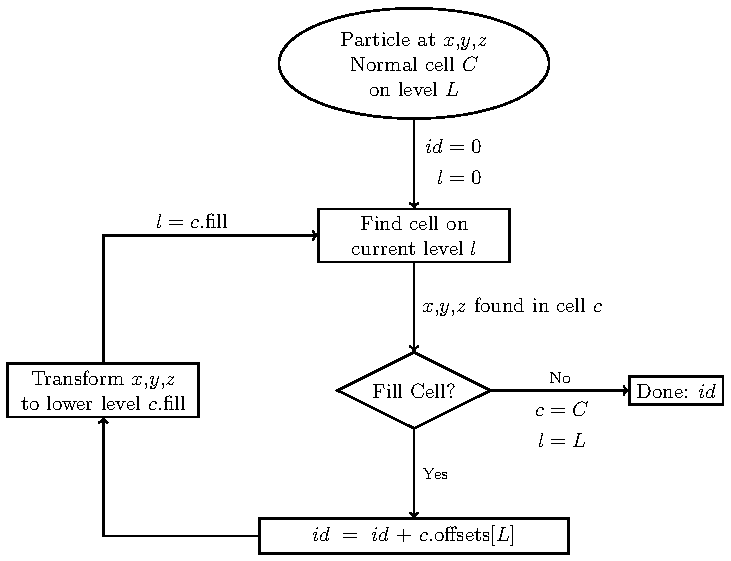
\includegraphics[width=6in]{figures/workflow/openmc/flow.pdf}
    \caption{\label{fig:indexing_scheme} Example geometry with 3 universe levels.  Material cells are defined in pin-cell universes $a$ and $b$, which are filled into the cells of lattice universes $B$ and $C$, which are filled into the cells of lattice universe $A$.  The colored numbers in each fill cell are the offsets for each base universe, which can be used to quickly compute a unique ID for each instance of a material cell.}
\end{figure}

\begin{figure}[htb!]
    \centering
    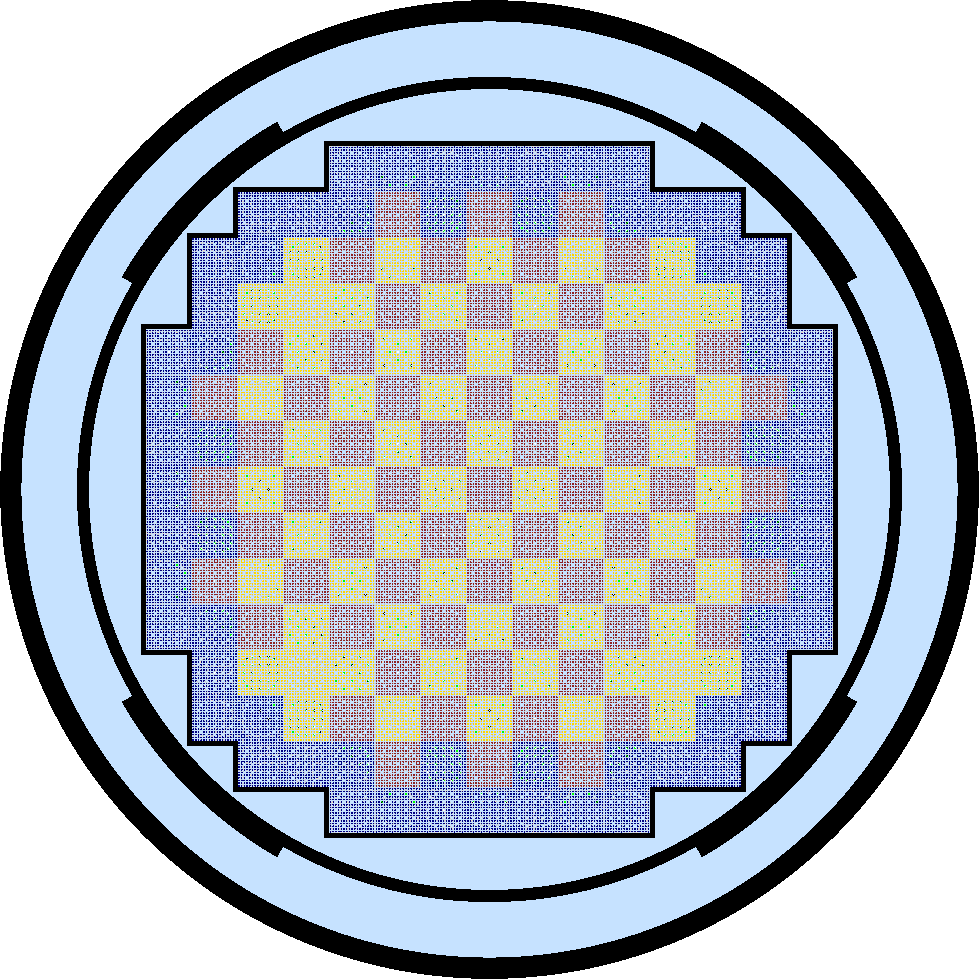
\includegraphics[width=2in]{figures/workflow/openmc/core}\hspace{1cm}
    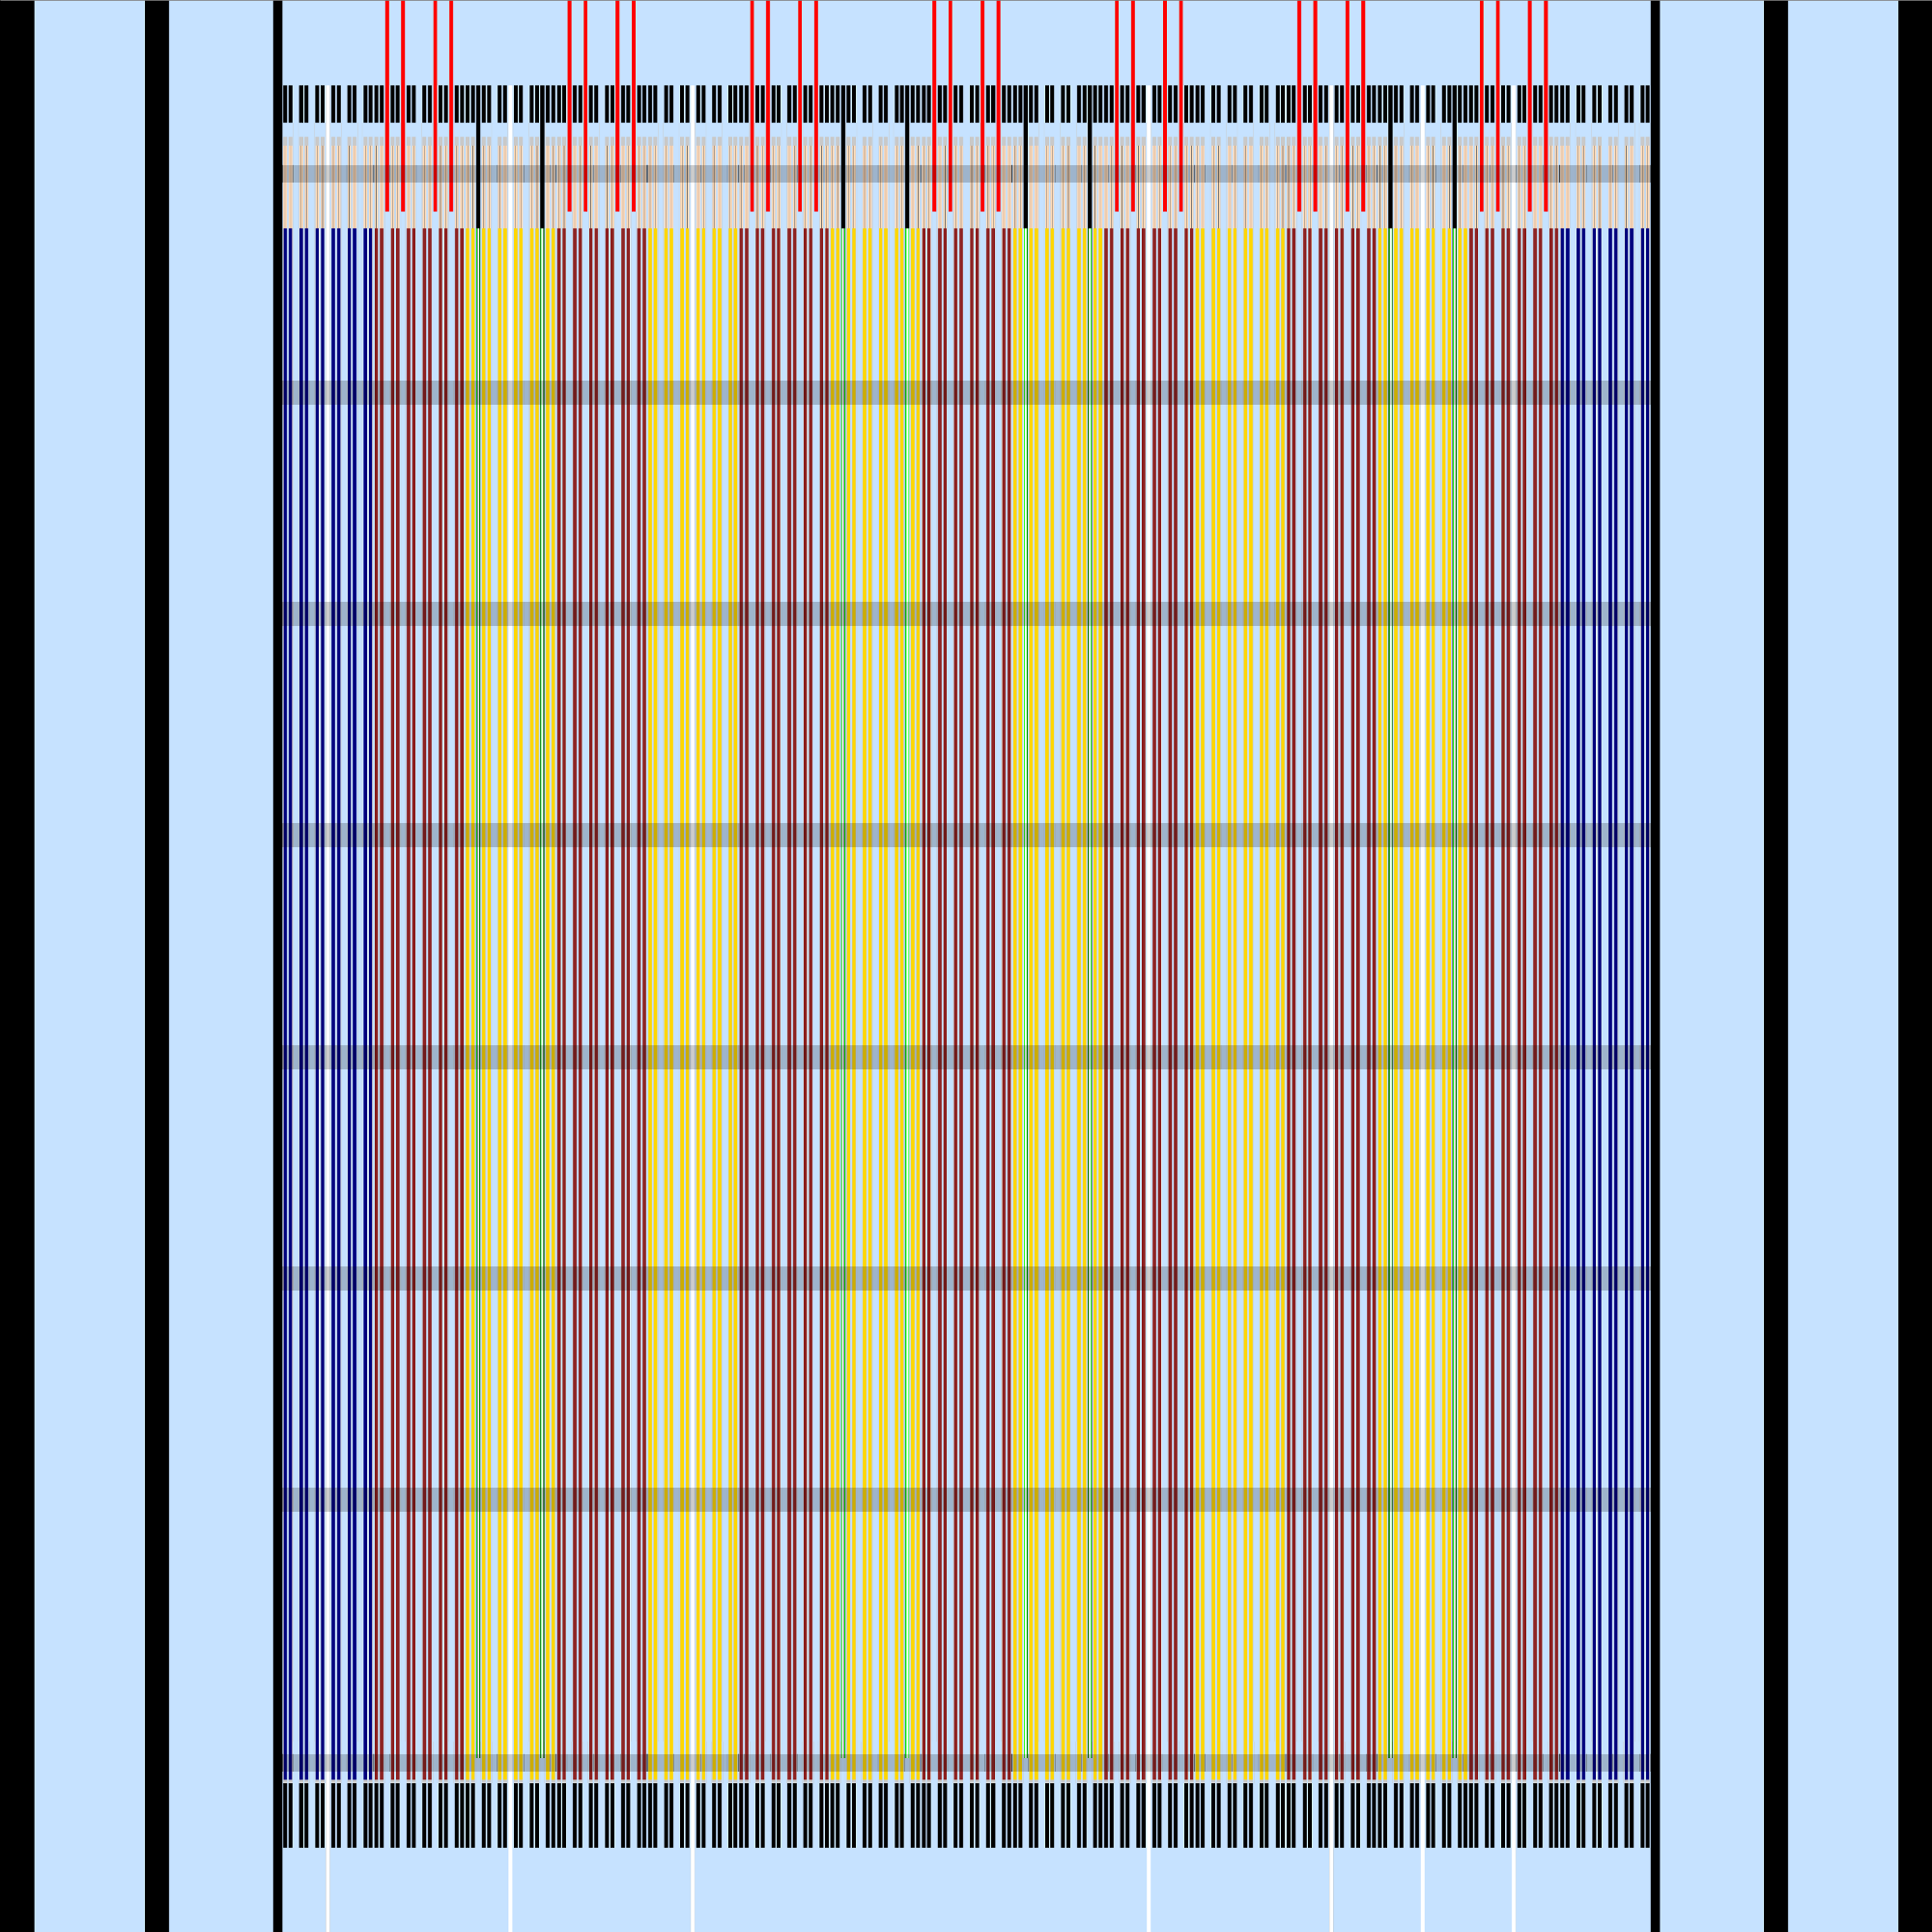
\includegraphics[width=2in]{figures/workflow/openmc/core_axial}
    \caption{\label{fig:beavrs} Geometry of the BEAVRS benchmark. \emph{Left:} Radial view, showing 193 fuel assemblies, colored by enrichment. \emph{Right:} Axial view, showing grid spacers and axial pin-cell features.}
\end{figure}

%%%%%%%%%%%%%%%%%%%%%%%%%%%%
\subsection{MGXS Generation}
\label{sec:chap3-mgxs}

\begin{itemize}[noitemsep]
  \item Python \ac{API} software stacks together in \texttt{openmc.mgxs}
\end{itemize}

-perhaps a figure with 

%%%%%%%%%%%%%%%%%%%%%%%%%%%%%%%%%%%%%%%%
\subsection{Isotropic-in-Lab Scattering}
\label{sec:chap3-iso-in-lab}


%%%%%%%%%%%%%%%%%%%%%%%%%%%%%%%%%%%%%%%%%%%%%%%%%%%%%%%%%%%%%%%%%%%%%%%%%%%%%%%%
\section{OpenMOC}
\label{sec:chap3-openmoc}

\begin{itemize}[noitemsep]
  \item reference Annals paper~\cite{boyd2014openmoc}
  \item multi-core CPUs~\cite{boyd2016parallel} and GPUs~\cite{boyd2013massively}
  \item reference 3D \ac{MOC} papers
  \item brief description of \ac{MOC} equations
  \begin{itemize}[noitemsep]
    \item flat/linear source approx.
    \item isotropic approx.
    \item constant-in-angle \ac{MGXS}
    \item uses total/transport, nu-fission, (nu-)scattering matrix, chi
  \end{itemize}
\end{itemize}

\begin{figure*}[ht!]
  \begin{subfigure}[htb!]{0.32\textwidth}
    \centering
    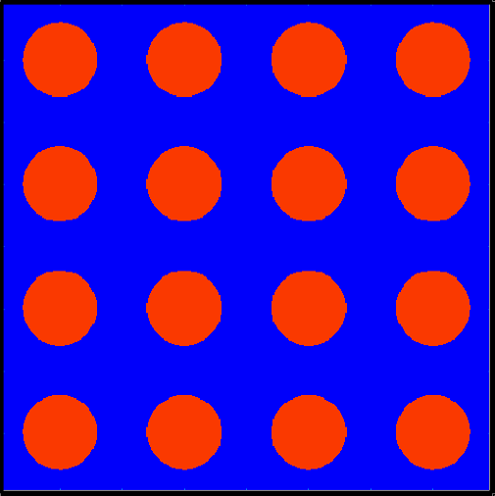
\includegraphics[width=0.95\textwidth]{figures/workflow/openmoc/materials-border}
    \label{fig:moc-model-materials}
    \caption{}
  \end{subfigure}
  \begin{subfigure}[htb!]{0.32\textwidth}
    \centering
    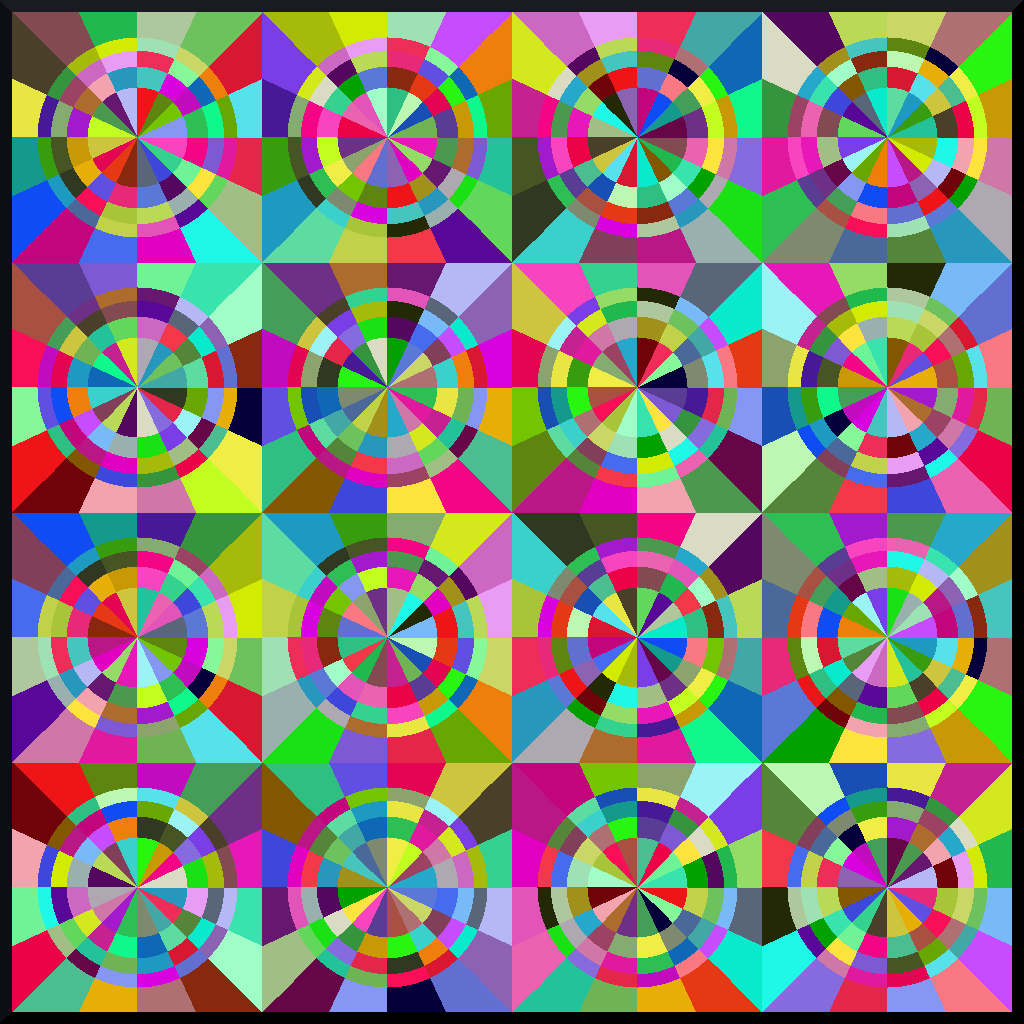
\includegraphics[width=0.95\textwidth]{figures/workflow/openmoc/FSRs}
    \label{fig:moc-model-fsrs}
    \caption{}
  \end{subfigure}
  \begin{subfigure}[htb!]{0.32\textwidth}
    \centering
    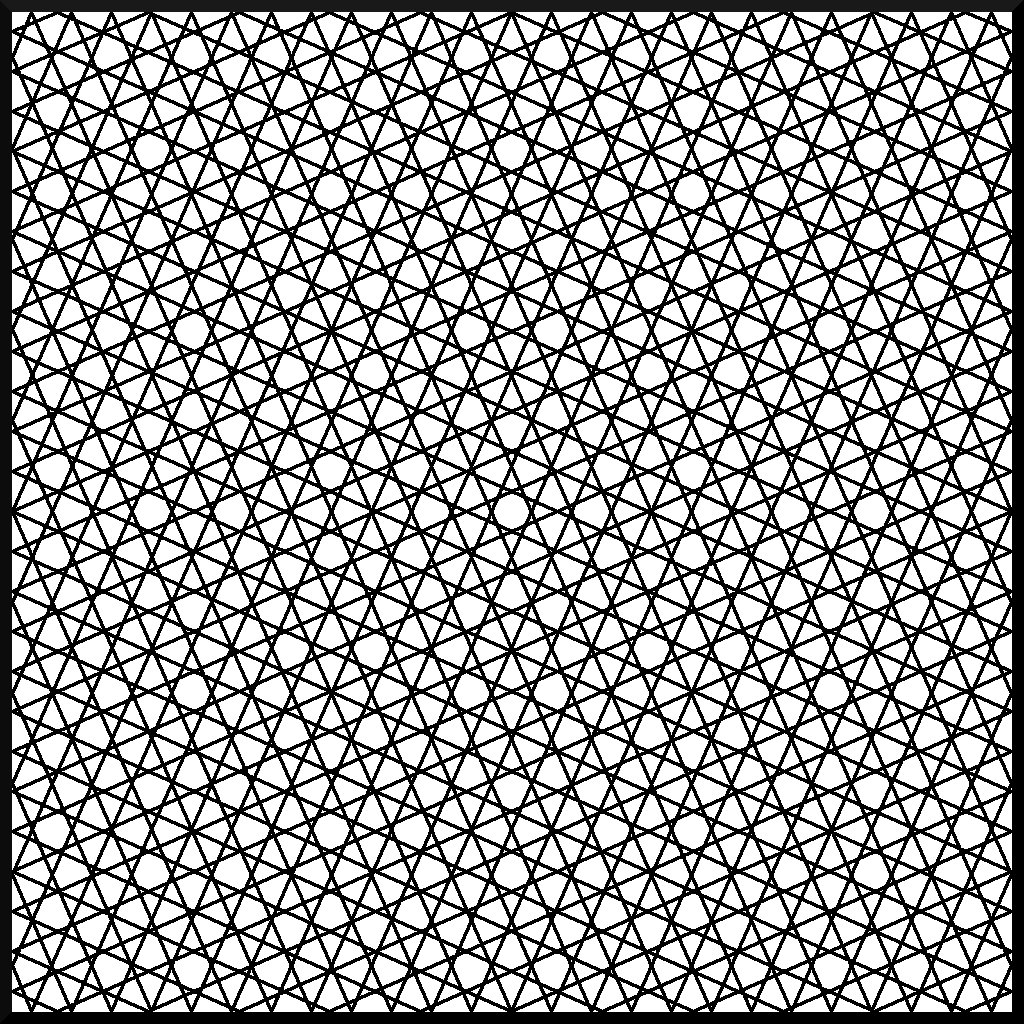
\includegraphics[width=0.95\textwidth]{figures/workflow/openmoc/cyclic-tracks}
    \label{fig:moc-model-tracks}
    \caption{}
  \end{subfigure}
\caption{The coolant and fuel materials (a), method of characteristics flat source region spatial mesh (b), and cyclic characteristic laydown (c) for a 4 $\times$ 4 fuel pin lattice.}
\label{fig:moc-model}
\end{figure*}


%%%%%%%%%%%%%%%%%%%%%%%%%%%%%%%%%%%%%%%%%%%%%%%%%%%%%%%%%%%%%%%%%%%%%%%%%%%%%%%%
\section{OpenCG}
\label{sec:chap3-opencg}

\begin{itemize}[noitemsep]
  \item single physics-agnostic geometries~\cite{boyd2015opencg}
  \item compatibility modules with OpenMC, OpenMOC
  \item ``glue'' code to map OpenMC distribcells to OpenMOC spatial mesh
\end{itemize}

\begin{figure}[h!]
  \centering
  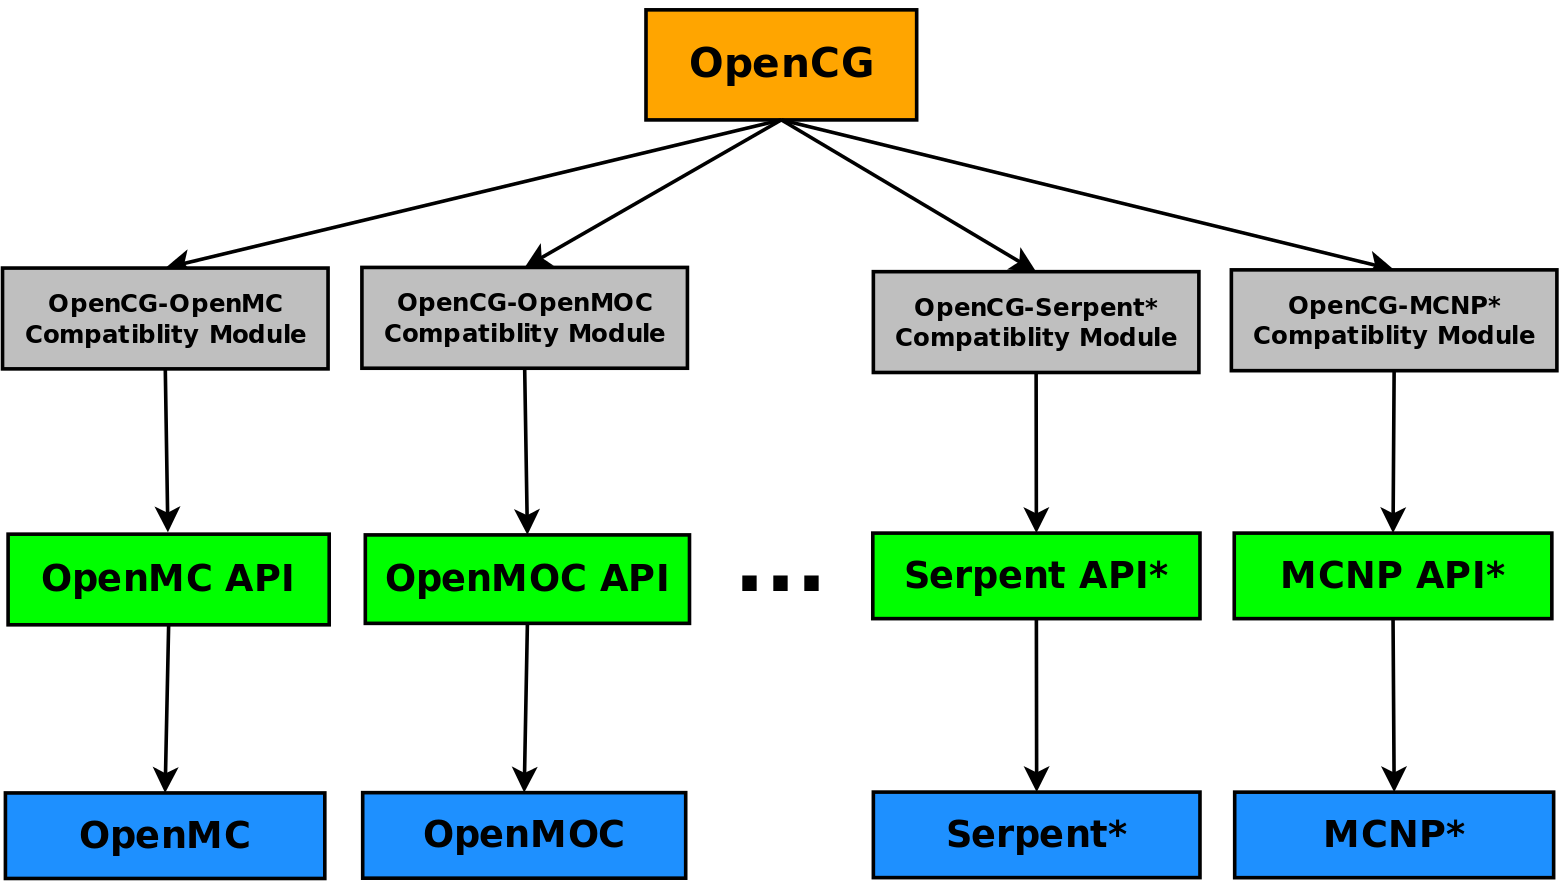
\includegraphics[width=.8\linewidth]{figures/workflow/opencg/compatibility-modules}
  \caption{OpenCG compatibility modules for various neutron transport codes. The compatibility modules for OpenMC and OpenMOC will be released in future public distributions of each code, while modules for Serpent and MCNP are in progress at the time of this writing.}
  \label{fig:compatibility-modules}
\end{figure}


%%%%%%%%%%%%%%%%%%%%%%%%%%%%%%%%%%%%
\subsection{Local Neighbor Symmetry}
\label{sec:chap3-lns}

\begin{algorithm}[h!]
\caption{Local Neighbor Symmetry Identification}
\label{alg:local-neighbor-symmetry-cells}
\begin{algorithmic}[1]
\Procedure{computeNeighborSymmetry}{$path$}
    \State $G \gets \emptyset$ \Comment{Initialize empty set for graph}
    \State $k \gets$ \textbf{length}($path$) \Comment{Find number of independent sets}
    \For{$i := 1, k$}
        \If{\textbf{type}($path[i]$) \textbf{is} UNIVERSE}
            \State $G \gets G \cup \{path[i]\}$ \Comment{Append universe to graph}
        \ElsIf{\textbf{type}($path[i]$) \textbf{is} LATTICE}
            \State $N \gets$ \Call{BreadthFirstSearch}{$path[i]$} \Comment{Find lattice cell neighbors}
            \State $G \gets G \cup \{N\}$ \Comment{Append neighbors to graph}
        \ElsIf{\textbf{type}($path[i]$) \textbf{is} CELL}
            \State $N \gets$ \Call{BreadthFirstSearch}{$path[i]$} \Comment{Find cell neighbors}
            \State $G \gets G \cup \{N\}$ \Comment{Append neighbors to graph}
        \EndIf
    \EndFor
    \State \textbf{return} \Call{Hash}{$G$} \Comment{Return $k$-partite graph hash}
\EndProcedure
\end{algorithmic}
\end{algorithm}

\begin{itemize}[noitemsep]
  \item analogy to lattice physics geometric templates based on eng. approx.
\end{itemize}

\begin{figure}
\begin{subfigure}{.5\textwidth}
  \centering
  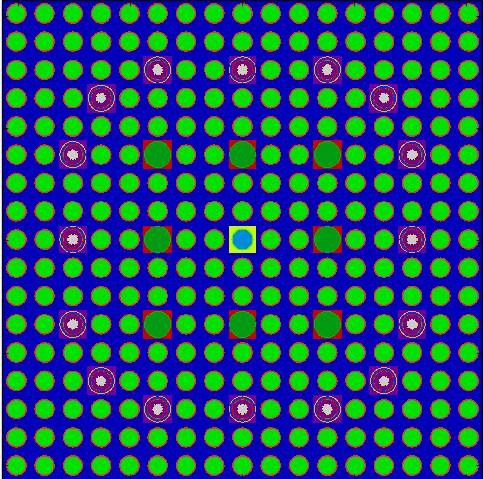
\includegraphics[width=.7\linewidth]{figures/workflow/opencg/cells-xy-24-16-assm}
  \caption{}
  \label{fig:assm-cells}
\end{subfigure}%
\begin{subfigure}{.5\textwidth}
  \centering
  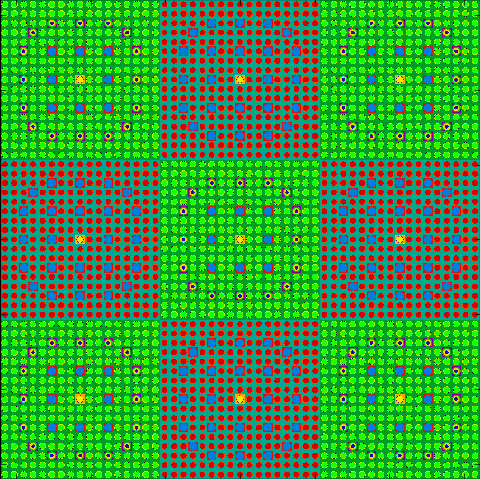
\includegraphics[width=.7\linewidth]{figures/workflow/opencg/cells-xy-colorset}
  \caption{}
  \label{fig:colorset-cells}
\end{subfigure}
\begin{subfigure}{.5\textwidth}
  \centering
  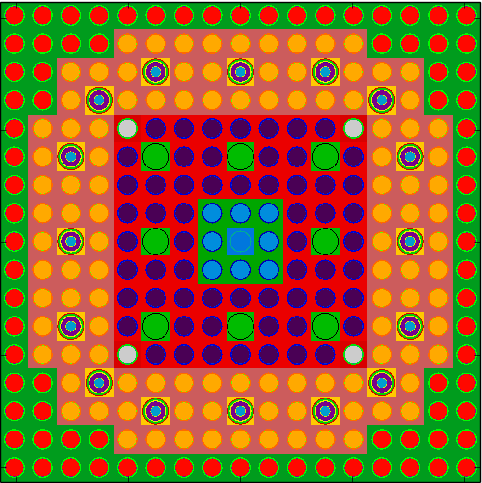
\includegraphics[width=.7\linewidth]{figures/workflow/opencg/unique-neighbor-cells-xy-24-16-assm}
  \caption{}
  \label{fig:assm-unique-neighbors}
\end{subfigure}
\begin{subfigure}{.5\textwidth}
  \centering
  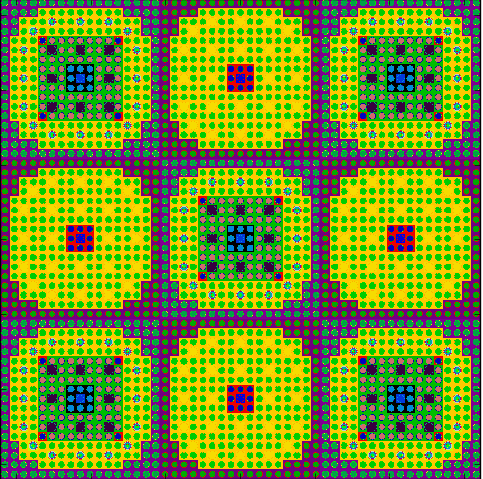
\includegraphics[width=.7\linewidth]{figures/workflow/opencg/unique-neighbor-cells-xy-colorset}
  \caption{}
  \label{fig:colorset-unique-neighbors}
\end{subfigure}
\begin{subfigure}{.5\textwidth}
  \centering
  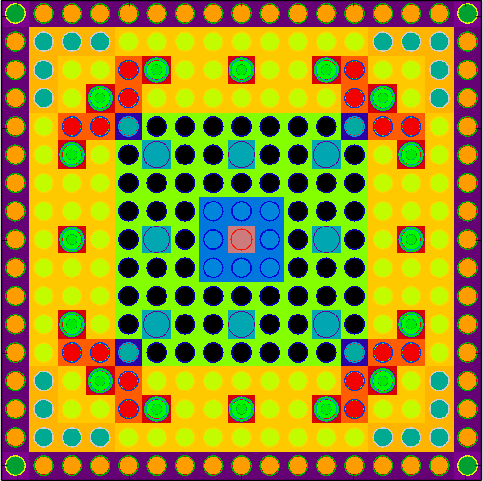
\includegraphics[width=.7\linewidth]{figures/workflow/opencg/neighbor-cells-xy-24-16-assm}
  \caption{}
  \label{fig:assm-neighbors}
\end{subfigure}
\begin{subfigure}{.5\textwidth}
  \centering
  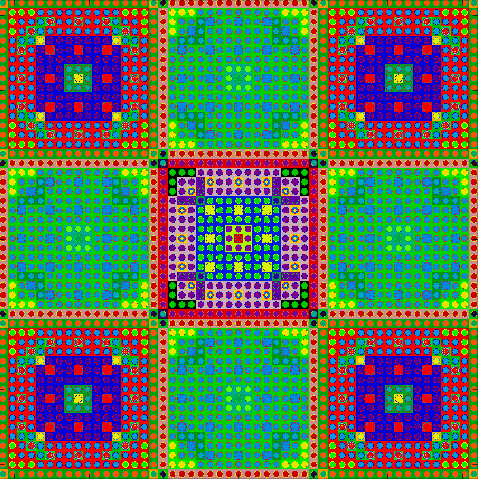
\includegraphics[width=.7\linewidth]{figures/workflow/opencg/neighbor-cells-xy-colorset}
  \caption{}
  \label{fig:colorset-neighbors}
\end{subfigure}
\caption{Two rectilinear lattice geometries are depicted to illustrate the use of local neighbor symmetry identification~\cite{boyd2015opencg}. The \textit{cells} are depicted for (a) a 17$\times$17 PWR lattice and (b) a 3$\times$3 colorset of two different 17 $\times$ 17 PWR assemblies each with burnable absorbers, guide tubes and instrument tubes. The \textit{unique neighbor} symmetry identifiers are color-coded in (c) and (d) for the assembly and colorset, respectively. Likewise, the \textit{general neighbor} symmetry identifiers are color-coded in (e) and (f).}
\label{fig:neighbor-cells}
\end{figure}

%%%%%%%%%%%%%%%%%%%%%%%%%%%%%%%%%%%%
\subsection{Region Differentiation}
\label{sec:chap3-region-diff}

\begin{itemize}[noitemsep]
  \item retain CSG's simplicity of repeated primitives for user input
  \item build combinatorial geometries based on arbitrary clustering of cell instances
\end{itemize}


\newpage
\begin{figure}[h!]
\begin{subfigure}{\textwidth}
  \centering
  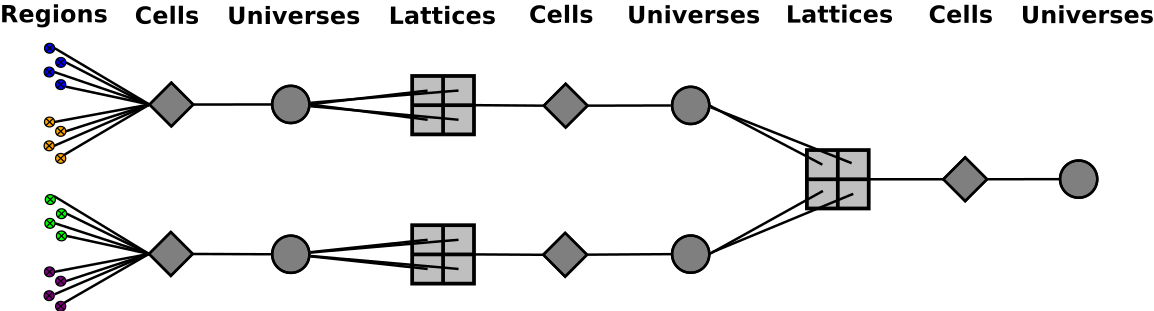
\includegraphics[width=0.82\linewidth]{figures/workflow/opencg/region-differentiation-1}
  \caption{}
  \label{fig:differentation-1}
\end{subfigure}
\begin{subfigure}{\textwidth}
  \centering
  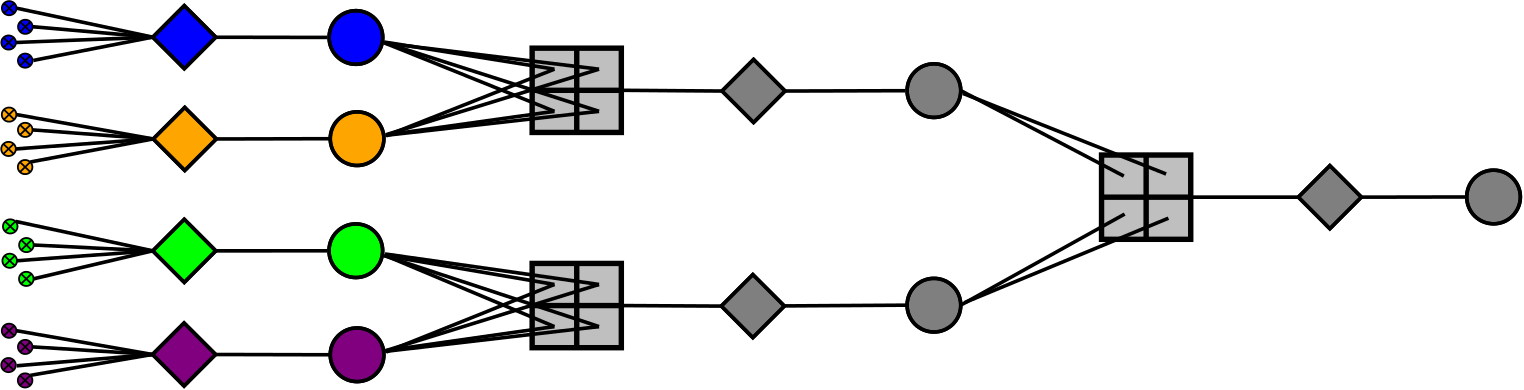
\includegraphics[width=0.75\linewidth]{figures/workflow/opencg/region-differentiation-2}
  \caption{}
  \label{fig:differentation-2}
\end{subfigure}
\begin{subfigure}{\textwidth}
  \centering
  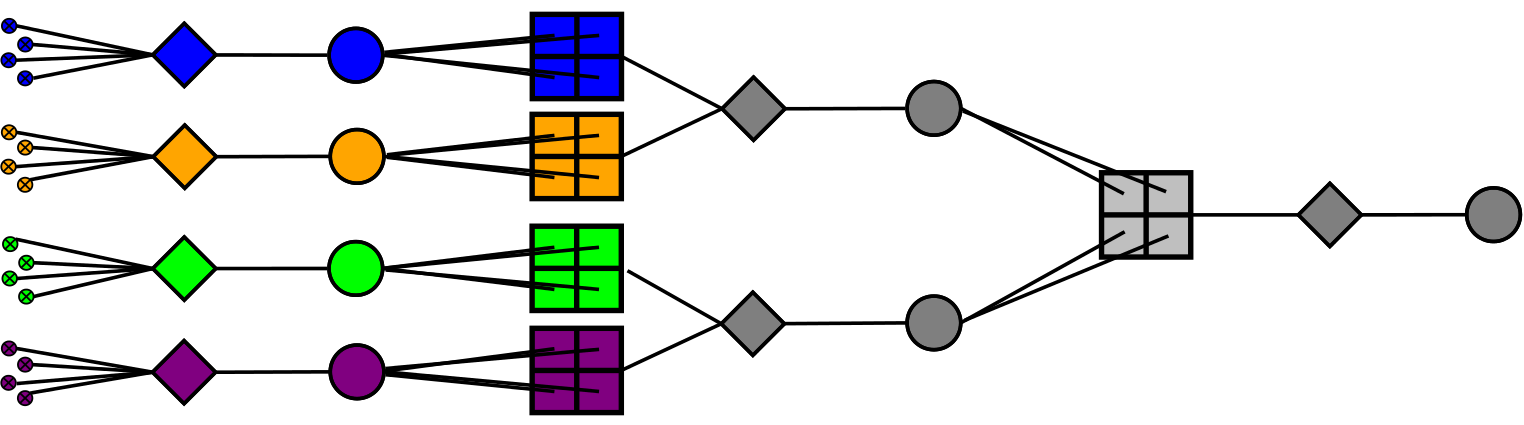
\includegraphics[width=0.75\linewidth]{figures/workflow/opencg/region-differentiation-3}
  \caption{}
  \label{fig:differentation-3}
\end{subfigure}
\begin{subfigure}{\textwidth}
  \centering
  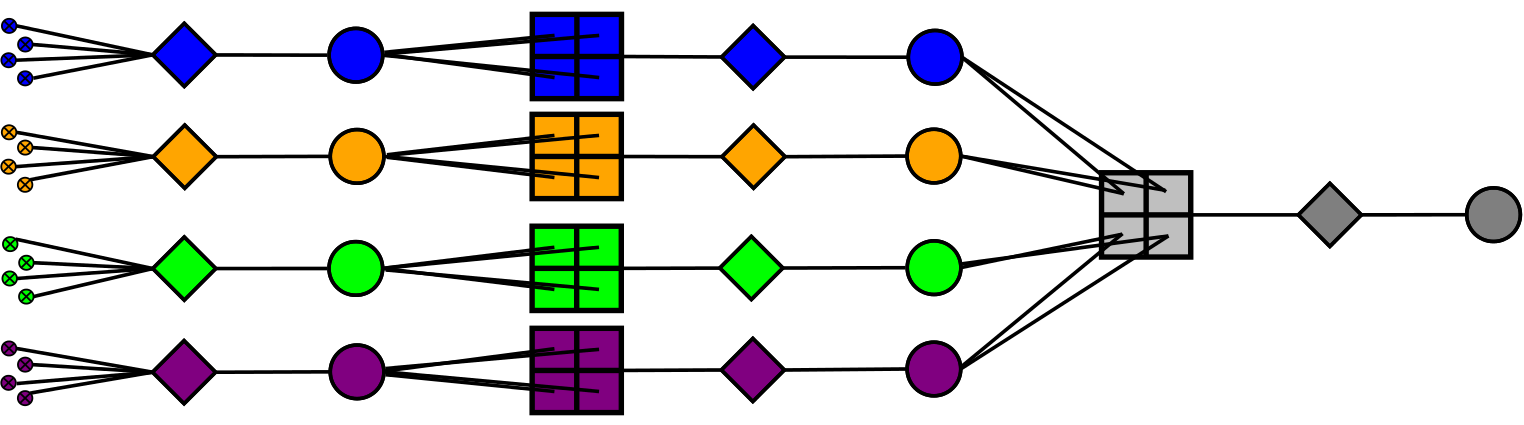
\includegraphics[width=0.75\linewidth]{figures/workflow/opencg/region-differentiation-4}
  \caption{}
  \label{fig:differentation-4}
\end{subfigure}
\begin{subfigure}{\textwidth}
  \centering
  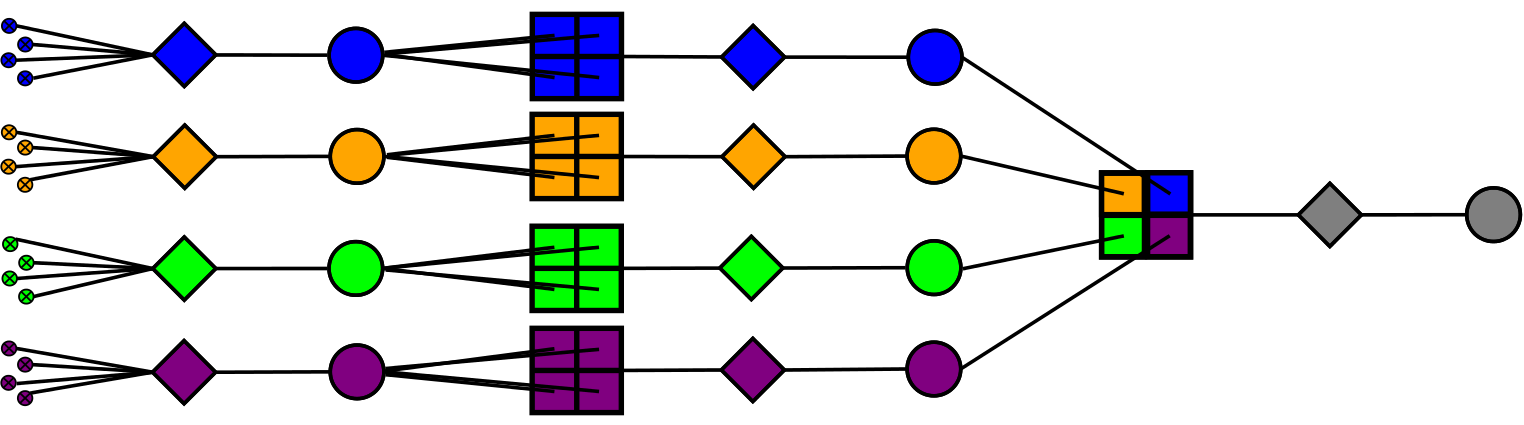
\includegraphics[width=0.75\linewidth]{figures/workflow/opencg/region-differentiation-5}
  \caption{}
  \label{fig:differentation-5}
\end{subfigure}
\caption{A few of the stages of the region differentiation algorithm~\cite{boyd2015opencg}. The regions (cell instances) to be differentiated are grouped and colored blue, orange, green and purple in (a). The first levels of cells and universes for each region group are differentiated in (b). The same is done for the lattices in (c). The algorithm continues to recursively differentiate cells, universes and lattices until no region groups collide at any level of the CG tree in (e).}
\label{fig:region-differentiation}
\end{figure}